%%%%%%%%%%%%%%%%%%%%%%%%%%%%%%%%%%%%%%%%%
% Geometria obliczeniowa
% Wyznaczanie minimalnego okręgu i prostokąta zawierającego chmurę punktów 2D 
%
%%%%%%%%%%%%%%%%%%%%%%%%%%%%%%%%%%%%%%%%%

%----------------------------------------------------------------------------------------
%	PACKAGES AND THEMES
%----------------------------------------------------------------------------------------

\documentclass{beamer}

\usepackage[T1]{fontenc}
\usepackage[polish]{babel}
\usepackage[utf8]{inputenc}
\usepackage{lmodern}
\usepackage{amsmath}

\selectlanguage{polish}

\mode<presentation> {
	\usetheme{Copenhagen}
}

\usepackage{graphicx} % Allows including images
\usepackage{booktabs} % Allows the use of \toprule, \midrule and \bottomrule in tables
\usepackage{gensymb}
\usepackage[shortlabels]{enumitem}

% Custom macros

\definecolor{links}{HTML}{2A1B81}
\hypersetup{colorlinks,linkcolor=,urlcolor=links}


%----------------------------------------------------------------------------------------
%	TITLE PAGE
%----------------------------------------------------------------------------------------

\title
[Minimalny okręg i prostokąt na chmurze punktów]
{Wyznaczanie minimalnego okręgu i prostokąta zawierającego chmurę punktów 2D}

\author
[Jakub Stępak]
{Jakub Stępak}

\institute
[AGH]
{
Akademia Górniczo – Hutnicza w Krakowie
}
\date{24 października 2016}

%----------------------------------------------------------------------------------------

\begin{document}

\frame{\titlepage}

%----------------------------------------------------------------------------------------
%	PRESENTATION SLIDES
%----------------------------------------------------------------------------------------

%------------------------------------------------
\section{Przedstawienie problemu}
%------------------------------------------------

\subsection{Przedstawienie problemu}

\begin{frame}

\frametitle{Problem}
Zadana jest chmura punktów na płaszczyźnie dwuwymiarowej.
\linebreak
\linebreak
Znaleźć:
\begin{itemize}[-]
\item najmniejszy \textbf{okręg} ją zawierący,
\item prostokąt ją zawierający o minimalnym \textbf{polu},
\item prostokąt ją zawierający o minimalnym \textbf{obwodzie}.
\end{itemize}

\end{frame}

%------------------------------------------------

\subsection{Otoczka wypukła}

\begin{frame}

Wszystkie rozwiązania będą opierały się o wyznaczoną otoczkę wypukłą zadanej chmury punktów. 
\linebreak 
\linebreak
Otoczkę wyznaczamy, na przykład, algorytmem Grahama.

\end{frame}

%------------------------------------------------

\section{Rozwiązanie}

\subsection{Algorytm Appleta}

\begin{frame}
\frametitle{Najmniejszy okręg}
\begin{center}
Do znalezienia najmniejszego okręgu użyjemy \textbf{algorytmu Appleta}.
\end{center}

\end{frame}

%------------------------------------------------

\begin{frame}
\frametitle{Obserwacja}
\begin{center}
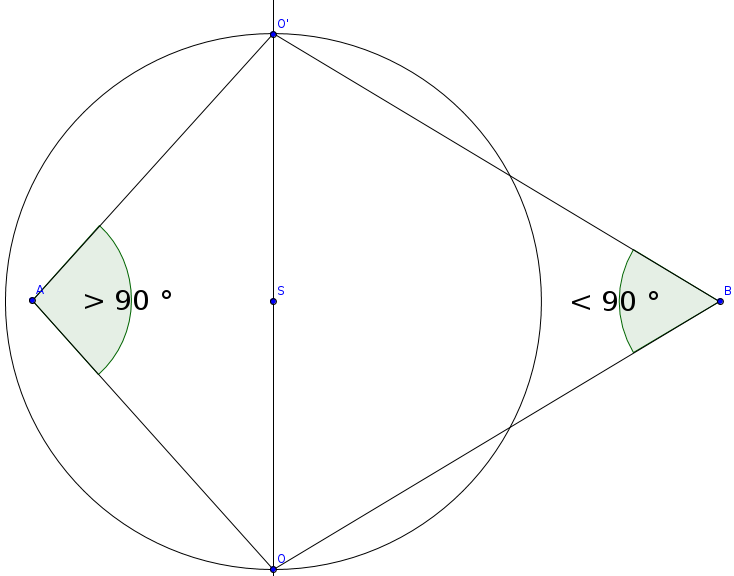
\includegraphics[width=0.65\paperwidth]{pics/angles.png}
\end{center}

\end{frame}

%------------------------------------------------

\begin{frame}

\frametitle{Algorytm Appleta}

\begin{enumerate}[1.]

\item Wybierzmy dowolną krawędź otoczki $S  = [P_1, P_2]$.

\item Dla każdego wierzchołka $P_0 \neq P_1, P_2$, 
obliczamy $ \measuredangle P_1 P_0 P_2 $. 

\item Najmniejszy znaleziony kąt oznaczmy przez $\alpha$, 
a wierzchołek przy którym występuje przez $V$:

\begin{enumerate}[a)]

\item Jeśli $ \alpha > 90 \degree $ to rozwiązaniem jest okrąg opisany na $S$. 
\item  Jeśli $ \alpha < 90 \degree $ sprawdzamy pozostałe 
kąty $ \triangle P_1 V P_2 $:

\begin{enumerate}[-]
\item  Jeśli żaden nie jest rozwarty, to rozwiązaniem 
jest okrąg opisany na $ \triangle P_1 V P_2 $.

\item Jeśli któryś z kątow jest rozwarty, krawędź na przeciwko niego 
staje się nowym $S$. Wracamy do punktu 2.

\end{enumerate}

\end{enumerate}

\end{enumerate}

\end{frame}

%------------------------------------------------

\begin{frame}

\frametitle{Przykład 1}
\begin{center}
\includegraphics[width=0.80\paperwidth]<1>{pics/halfcircle/000.png}
\includegraphics[width=0.80\paperwidth]<2>{pics/halfcircle/001.png}
\includegraphics[width=0.80\paperwidth]<3>{pics/halfcircle/002.png}
\includegraphics[width=0.80\paperwidth]<4>{pics/halfcircle/003.png}
\includegraphics[width=0.80\paperwidth]<5>{pics/halfcircle/004.png}
\includegraphics[width=0.80\paperwidth]<6>{pics/halfcircle/005.png}
\includegraphics[width=0.80\paperwidth]<7>{pics/halfcircle/006.png}
\includegraphics[width=0.80\paperwidth]<8>{pics/halfcircle/007.png}
\end{center}

\end{frame}

%------------------------------------------------

\begin{frame}

\frametitle{Przykład 2}
\begin{center}
\includegraphics[width=0.65\paperwidth]<1>{pics/circle/000.png}
\includegraphics[width=0.65\paperwidth]<2>{pics/circle/001.png}
\includegraphics[width=0.65\paperwidth]<3>{pics/circle/002.png}
\includegraphics[width=0.65\paperwidth]<4>{pics/circle/003.png}
\includegraphics[width=0.65\paperwidth]<5>{pics/circle/004.png}
\includegraphics[width=0.65\paperwidth]<6>{pics/circle/005.png}
\end{center}

\end{frame}

%------------------------------------------------

\subsection{Najmniejszy prostokąt}

\begin{frame}
\frametitle{Wyszukiwanie najmniejszego prostokąta}
\begin{enumerate}[1)]
\item „Obróć” otoczką, „kładąc” ją na kolejnym boku na osi OX.
\item Oblicz pole i obwód prostokąta utworzonego przez skrajne punkty (z największą i najmnięjszą współrzędną x i y)
\item Zapamiętaj które prostokąty był najmniejszy.
\end{enumerate}

\end{frame}

%------------------------------------------------

\begin{frame}
\frametitle{Prostokąt o najmniejszym polu i obwodzie to nie zawsze ten sam prostokąt!}

\begin{center}
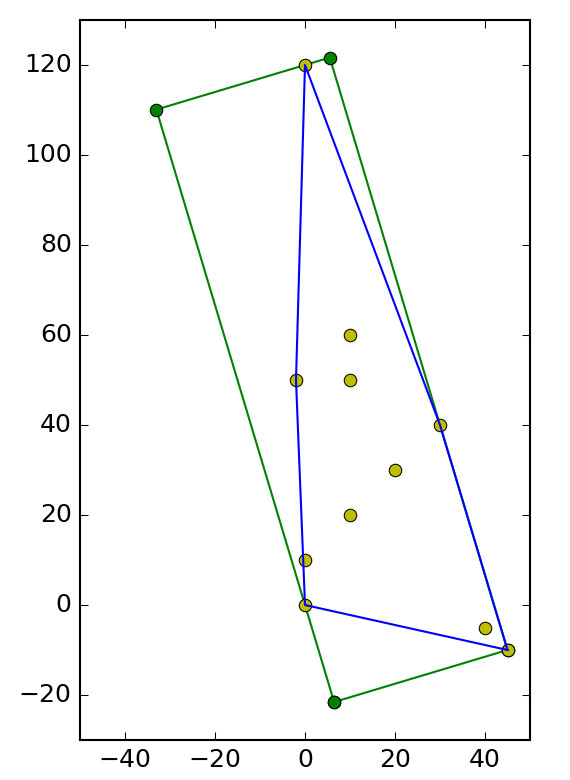
\includegraphics[height=0.65\paperheight]{pics/area.png}
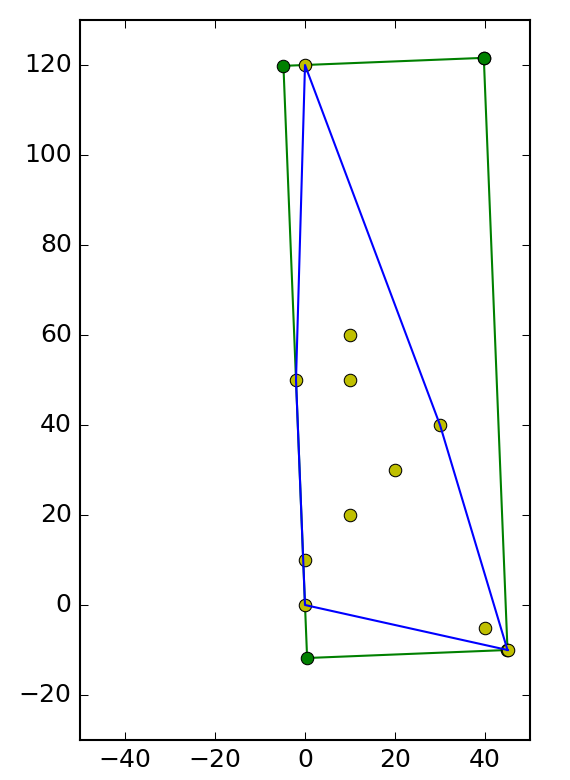
\includegraphics[height=0.65\paperheight]{pics/perim.png}
\end{center}

\end{frame}

%------------------------------------------------

\begin{frame}

\frametitle{Przykład - najmniejsze pole}
\begin{center}
\includegraphics[width=0.70\paperwidth]<1>{pics/area/000.png}
\includegraphics[width=0.70\paperwidth]<2>{pics/area/001.png}
\includegraphics[width=0.70\paperwidth]<3>{pics/area/002.png}
\includegraphics[width=0.70\paperwidth]<4>{pics/area/003.png}
\includegraphics[width=0.70\paperwidth]<5>{pics/area/004.png}
\includegraphics[width=0.70\paperwidth]<6>{pics/area/005.png}
\includegraphics[width=0.70\paperwidth]<7>{pics/area/006.png}
\includegraphics[width=0.70\paperwidth]<8>{pics/area/007.png}
\includegraphics[width=0.70\paperwidth]<9>{pics/area/008.png}
\includegraphics[width=0.70\paperwidth]<10>{pics/area/009.png}
\includegraphics[width=0.70\paperwidth]<11>{pics/area/010.png}
\includegraphics[width=0.70\paperwidth]<12>{pics/area/011.png}
\includegraphics[width=0.70\paperwidth]<13>{pics/area/012.png}
\includegraphics[width=0.70\paperwidth]<14>{pics/area/013.png}
\end{center}

\end{frame}

%------------------------------------------------

\begin{frame}

\frametitle{Przykład - najmniejszy obwód}
\begin{center}
\includegraphics[width=0.70\paperwidth]<1>{pics/perimeter/000.png}
\includegraphics[width=0.70\paperwidth]<2>{pics/perimeter/001.png}
\includegraphics[width=0.70\paperwidth]<3>{pics/perimeter/002.png}
\includegraphics[width=0.70\paperwidth]<4>{pics/perimeter/003.png}
\includegraphics[width=0.70\paperwidth]<5>{pics/perimeter/004.png}
\includegraphics[width=0.70\paperwidth]<6>{pics/perimeter/005.png}
\includegraphics[width=0.70\paperwidth]<7>{pics/perimeter/006.png}
\includegraphics[width=0.70\paperwidth]<8>{pics/perimeter/007.png}
\includegraphics[width=0.70\paperwidth]<9>{pics/perimeter/008.png}
\includegraphics[width=0.70\paperwidth]<10>{pics/perimeter/009.png}
\includegraphics[width=0.70\paperwidth]<11>{pics/perimeter/010.png}
\includegraphics[width=0.70\paperwidth]<12>{pics/perimeter/011.png}
\includegraphics[width=0.70\paperwidth]<13>{pics/perimeter/012.png}
\includegraphics[width=0.70\paperwidth]<14>{pics/perimeter/013.png}
\end{center}

\end{frame}

%------------------------------------------------

\begin{frame}
\frametitle{Koniec}

\begin{center}
Dziękuję za uwagę
\end{center}

\begin{center}
Prezentacja oraz kod programu dostępne na moim GitHubie:
\url{https://github.com/jakubste/geo-project}
\end{center}


\end{frame}

%------------------------------------------------

\end{document} 
